\chapter{Technologien}

In diesem Kapitel wird ein Überblick über die Technologien gegeben, die zum Implementieren der Prototypen zu den Interaktionskonzepten genutzt wird.
Dabei wird auf der Hardwareseite auf das verwendete Anzeigegerät für AR, die Meta Quest 3, eingegangen, während auf Softwareseite die Engine und Frameworks vorgestellt werden, in welchen die Prototypen implementiert werden.

\section{Meta Quest 3}

Im Laufe der Bachelorarbeit wird als Anzeigegerät für die AR-Anwendung die Meta Quest 3 verwendet.
Dabei handelt es sich um ein Standalone-AR- und VR-Headset, welches von Meta (ehemals Facebook) entwickelt wurde und Ende 2023 auf den Markt kam.
Das HMD ist mit einem eigens für mobile XR-Geräte entwickelten Qualcomm Snapdragon XR2 Gen2 Prozessor ausgestattet, der speziell für VR- und AR-Anwendungen entwickelt wurde, und ist dadurch selbst in der Lage auch anspruchsvolle Inhalte zu rendern.
Es muss nicht wie viele andere HMDs an einen Computer oder ein Smartphone angeschlossen werden, sondern kann direkt verwendet werden.
Das Headset verfügt auch beispielsweise über einen eigenen Browser, wodurch AR Anwendungen auch einfach übers Internet aufgerufen werden können.
Dieses Nutzern von Anwendungen über den Browser wird auch für die Prototypen dieser Arbeit genutzt, worauf in Kapitel \ref{section:webxr} genauer eingegangen wird.

Über zwei Displays mit jeweils einer Auflösung von 2064 x 2208 Pixeln und einer Bildwiederholrate von bis zu 120Hz zeigt das Headset Inhalte mit einer hohen Bildqualität und einer flüssigen Darstellung an.
Durch die Kombination der geringen Latenz aufgrund des On-Board-Prozessors und der hohen Bildwiederholrate sollte das Gerät eine hohe Immersion und ein angenehmes Nutzungserlebnis bieten.

\newpage

Darüber hinaus verfügt die Oculus Quest 3, wie auf Abbildung \ref{fig:quest-front-cameras} zu sehen ist, über zwei RGB-Kameras (untere Kameras), zwei IR-Kameras (obere Kameras) sowie einen Tiefenprojektor (schwarze Fläche in der Mitte) auf der Vorderseite, welche die Umgebung des Nutzers erfassen können und so AR-Anwendungen mittels Image-Passthrough ermöglichen.

\begin{figure}[H]
  \centering
  \includegraphics[width=0.7\textwidth]{images/Oculus-FrontCameras.jpg}
  \caption{Frontal ausgerichtete Kameras und Tiefenprojektor der Oculus Quest 3}
  \label{fig:quest-front-cameras}
\end{figure}

Zusätzlich zu den 2 RGB-Kameras sind insgesamt noch 4 Infrarot-Kameras auf dem Headset verbaut, zwei davon auf der Vorderseite, direkt über den RGB-Kameras, und zwei auf der Unterseite.
Über diese Kameras wird auch die Position des Nutzers im Raum kontinuierlich getrackt und angepasst, sodass für das Headset keine externen Trackingstationen notwendig sind.

Die Meta Quest kann zudem alternativ zu Controllern als Eingabegeräte kann das Headset mithilfe der 4 IR-Kameras und 2 RGB-Kameras die Hände des Nutzers erkennen und tracken, sodass die eigenen Hände in VR- und AR-Anwendungen als Eingabegerät verwendet werden können \autocite[]{meta-quest-3}.
Dafür sind zwei der vier Infrarotkameras wie in Abbildung \ref{fig:quest-hand-cameras} zu sehen ist nach unten gerichtet, um die Hände des Nutzers jederzeit tracken zu können.

\begin{figure}[H]
  \centering
  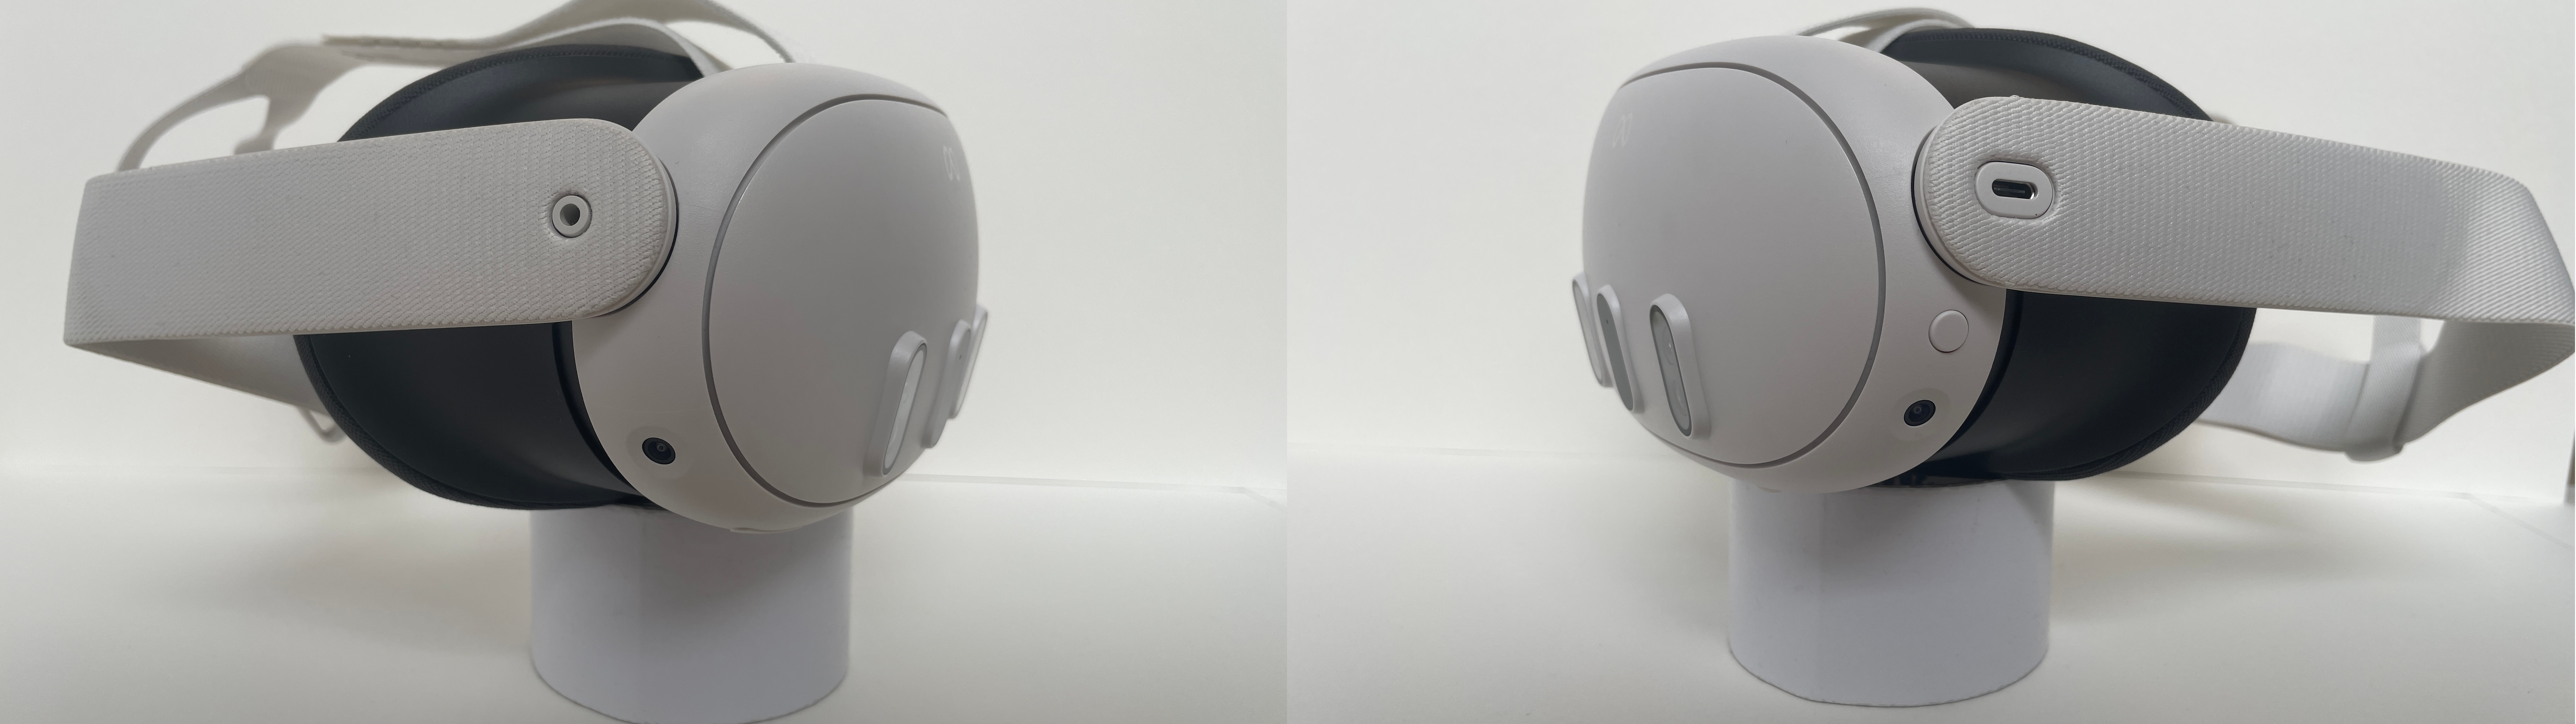
\includegraphics[width=1\textwidth]{images/Oculus_DownCameras.png}
  \caption{Die beiden nach unten gerichteten Kameras der Oculus Quest 3}
  \label{fig:quest-hand-cameras}
\end{figure}


\section{WebGL}

WebGL ist eine JavaScript-API, die das Rendern von 3D-Grafiken in einem Webbrowser ermöglicht.
Die WebGL-Spezifikation wird von der Khronos Group entwickelt, einer Non-Profit-Organisation, welche als ein Zusammenschluss aus über 180 Unternehmen aus der Tech-Industrie technologische Standards entwickelt.
Darunter sind auch die Unternehmen hinter den größten Browsern der Industrie: Google (Chrome), Mozilla (Firefox), Apple (Safari) und Microsoft (Edge) \autocite[]{khronos-webgl, khronos-about}.
Aufgrund dieser Mitarbeit verschiedener Unternehmen und der offenen Entwicklung der Spezifikation kann WebGL in fast allen modernen Webbrowsern verwendet werden.

WebGL basiert dabei auf der OpenGL ES Spezifikation, welche, ebenfalls von der Khronos Group, speziell für Embedded Systems und mobile Systeme, also zum Großteil Systeme ohne eigene Grafikkarte, entwickelt wurde \autocite[]{khronos-opengles}.
Aufgrund dieser Ausrichtung auf mobile Geräte, können mit WebGL Anwendungen entwickelt werden, die auf einfachen Geräten wie Smartphones oder aber auch auf VR- und AR-Headsets ohne zusätzliche Rechenleistung laufen \autocite[][S.3]{Baruah2021}.


\section{WebXR}
\label{section:webxr}

WebXR ist eine standardisierte API für Webanwendungen, welche es ermöglicht, immersive VR und AR Anwendungen für das Internet zu erstellen.
Das World Wide Web Consortium (W3C), welches die WebXR-Standards definiert beschreibt WebXR wie folgt: \glqq{}Die WebXR Device API bietet die notwendigen Schnittstellen, damit Entwickler ansprechende, komfortable und sichere immersive Anwendungen im Web für eine Vielzahl von Hardware-Formfaktoren erstellen können.\grqq{} \autocite[aus dem Englischen mit DeepL ][1. Introduction]{w3c_webxr}
Mit WebXR entwickelte Anwendungen können als Webanwendungen direkt von einem Webbrowser eines AR- oder VR-Geräts aus aufgerufen werden, ohne dass eine zusätzliche Installation der Anwendung notwendig ist.

\begin{figure}[H]
    \centering
    \includegraphics[width=0.6\textwidth]{images/WebXR-App-Flow.png}
    \caption{Application Flow von WebXR-Anwendungen}
    \source{nach \autocite[][Kap. 1.2. Application Flow]{w3c_webxr}}
    \label{fig:webxr-app-flow}
\end{figure}

Der Flow von WebXR-Anwendungen ist in Abbildung \ref{fig:webxr-app-flow} dargestellt.
Dabei wird zuerst beim Aufrufen der Anwendung geprüft, ob die angegebene Art von XR-Inhalt von der Hardware und dem User Agent (UA) unterstützt werden.
Mit dem User Agent (UA) der Software, ist dabei die Software gemeint, mit welcher der Nutzer auf die Anwendung zugreift, also der Webbrowser des Nutzers.
Ist die Art des XR-Inhalts von der Technik des Nutzers unterstützt, kann die XR-Session vom Nutzer manuell über einen Knopf gestartet werden.
Startet die Session erfolgreich, wird der Frame Loop der Anwendung gestartet.
Der Frame Loop ist eine Schleifenfunktion, die kontinuierlich während der XR-Session ausgeführt wird um die einzelnen Frames, bzw. Bilder, für das XR-Display zu rendern.
Dieser Frame Loop läuft, bis die Session durch den UA beendet wird.
Befindet sich der UA noch auf der Seite der WebXR-Anwendung, wird wieder der Knopf zum Starten der XR-Session angezeigt, falls der Nutzer direkt wieder eine neue Session starten möchte.

\subsection{Three.js}

Three.js ist eine Open-Source JavaScript-Bibliothek unter der MIT-Lizenz, die auf WebGL basiert und die Erstellung und Darstellung von 3D-Grafiken in Webanwendungen vereinfacht.
Die Bibliothek bietet eine Vielzahl von Funktionen, die es Entwicklern ermöglichen, detaillierte 3D-Modelle und -Szenen zu erstellen und zu rendern \autocite[][]{threejs-docs}.
Dabei unterstützt Three.js auch die Erstellung von AR- und VR-Anwendungen mithilfe von WebXR.

Es existieren auch einige Frameworks die auf der Three.js API basieren und die Entwicklung von AR- und VR-Anwendungen und 3D-Anwendungen generell weiter vereinfachen.
Ein Beispiel dafür ist das Framework A-Frame, welches auf die Entwicklung von AR und VR Anwendungen spezialisiert ist und Features einer fast vollwertigen Game-Engine bietet \autocite[]{a-frame-introduction}.

Zudem wird Three.js von vielen Entwicklern und Unternehmen verwendet und hat dadurch eine große Community und so viele Ressourcen und Tutorials, die Entwicklern helfen können, ihre Anwendungen zu erstellen und zu debuggen.

Diese Vielfalt an Features und die große Community machen Three.js, vor allem in Kombination mit A-Frame, zu einer interessanten Option für die Entwicklung von AR- und VR-Anwendungen.
Jedoch ergaben sich in den ersten Tests der Funktionalität von Three.js und A-Frame im Browser der Oculus Quest 3 Probleme mit der Erkennung der VR-Brille und der Darstellung von AR-Inhalten.

\subsection{Babylon.js}

Babylon.js ist eine Open-Source Rendering- und Game-Engine verpackt in einer JavaScript-Bibliothek die unter Anderem von einem Team von Entwicklern bei Microsoft entwickelt wird.
Es bietet Support für WebGL 1.0/2.0 sowie WebGPU und hat eine Vielzahl von Funktionen, die es Entwicklern ermöglichen, detaillierte 3D-Modelle und -Szenen zu erstellen und zu rendern.
Außerdem bietet es native Unterstützung und eine Dokumentation für WebXR, wodurch die Entwicklung von VR- und AR-Anwendungen vereinfacht wird \autocite[][]{babylon-features}.

Die Bibliothek bietet dabei auch viele Quality-of-Life-Features, wie beispielsweise einen Szenen-Explorer und -Inspektor, der sich für die Entwicklung und das Debugging von 3D-Szenen eignet und mit einer Zeile Code in die Anwendung eingebunden werden kann.
Über den Szenen-Explorer, welcher in Abbildung \ref{fig:babylon-inspector} links dargestellt ist, können aus dem Szenengraph der aktuellen Szene Objekte ausgewählt werden um im Szenen-Inspektor eine Detailansicht des Objekts und seinen Eigenschaften zu erhalten.
Mithilfe des Szenen-Inspektors, welcher in Abbildung \ref{fig:babylon-inspector} rechts dargestellt ist,  können dann in Echtzeit die Eigenschaften von Objekten betrachtet und verändert werden.

\begin{figure}[H]
  \centering
  \includegraphics[width=1\textwidth]{images/Babylon-Inspector.png}
  \caption{Szenen-Explorer und -Inspektor von Babylon.js}
  \label{fig:babylon-inspector}
\end{figure}
